%!TEX root = synchrony.tex

\section{Omitted Proofs}

\subsection{Proof of Lemma \ref{imposs:1}} \label{app:imposs:1}
\begin{proof}
\begin{figure}[h]
  \centering
  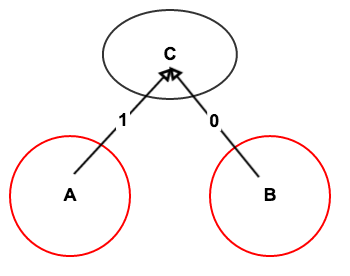
\includegraphics[scale=0.35]{impossible1.png}
  \caption{Case $m \geqslant d$  }
\end{figure}\label{sc1}

  The case $n=2$ is trivial. We assume $n \geqslant 3$.
  Suppose that $F$ is a $k$-round interactive consistency algorithm. Since $n \leqslant
  2m+d$, $P$ can be partitioned into three nonempty sets $A$, $B$, and $C$,
  with $| A | \leqslant m$, $| B | \leqslant m$, $| C | \leqslant d$. 
  
  We define two scenarios $\alpha$ and $\beta$.
  In $\alpha$, all processes have 0 as initial values.
  Processes in $B$ are faulty and send  to $C$ processes messages
  pretending that processes in $A$ have 1 as initial value.
  
   In $\beta$, processes in $A$ have 1 as initial value and all  others processes have 0 as initial value.
  Processes in $A$ are faulty and send to $C$ messages 
  pretending that processes in $A$ have 0 as initial value (see Figure~\ref{sc1}).
  
  In the two scenarios, processes in $C$ get the same messages, but in the first scenario 
  they have to decide 0 for processes in $A$ and $1$ in the second scenario leading to a contradiction.
    
More precisely  the scenarios $\alpha$
  and $\beta$ are defined as follows:
  \begin{enumerateroman}
    \item For every $w \in P^{+}$ not starting with a process of $A$, let
    \[ \alpha ( w ) = \beta ( w ) =0. \]
    \item For every $a \in A$, $b \in B$, $c \in C$ let
    \[ \alpha ( a ) = \alpha ( a a )  =  \alpha ( a b ) = \alpha ( a c )  = 0,
    \]
    \[ \beta ( a ) = \beta ( a a ) = \beta ( a b ) =1 \nocomma , \beta ( a c )
       =0. \]
    \item We define this part iteratively. 
    For every $a \in A$, $b \in B$, $c \in C$, $p \in P$, $w \in
    a P^{\ast}$, let
    \[ \alpha ( w c p ) = \alpha ( w c ) \nocomma , \alpha ( w a p ) = \alpha
       ( w a ) , \]
    \[ \beta ( w c p ) = \beta ( w c ) \nocomma , \beta ( w b p ) = \beta ( w
       b ) , \]
    \[ \alpha ( w b c ) = \beta ( w b ) \nocomma , \alpha ( w b a ) = \alpha
       ( w b ) , \]
    \[ \beta ( w a c ) = \alpha ( w a ) , \beta ( w a b )  =  \beta ( w a )
       . \]
  \end{enumerateroman}
  $\alpha$ is a  scenario in which processes in $B$ are faulty 
and  $\beta$ is a  scenario in which  faulty 
  processes are in set $A$. 
 Moreover,  $\alpha_{c} =
  \beta_{c}$ for all $c \in C$ then for any $a \in A$, $c \in C$
   \[ F_c ( \alpha_{c} )[a] = F_c ( \beta_{c} )[a].  \]

But for any $a \in A$, $c \in C$, as $F$ is a $k$-round  interactive consistency algorithm
    \[ F_c ( \alpha_{c})[a] = \alpha ( a ) = 0 , \] 
  \[ F_c ( \beta_{c} )[a] = \beta ( a ) =1 , \]
leading to a contradiction.
\end{proof}

\subsection{Proof of Lemma \ref{imposs:2}}\label{app:imposs:2}

\begin{proof}
\begin{figure}[h]
  \centering
  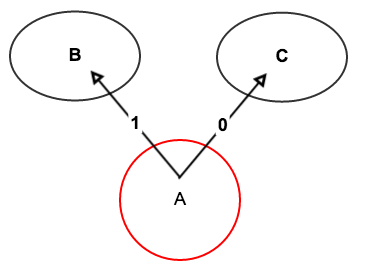
\includegraphics[scale=0.35]{impossible2.png}
  \caption{Case $d \geqslant m$  }
\end{figure}\label{sc2}

  This proof is similar to the proof above. 
  The case $n=2$ is trivial. We assume $n \geqslant 3$.
  Suppose that $F$ is a $k$-round  interactive
  consistency algorithm. Since $n \leqslant 2d+m$, $P$ can be partitioned into
  three non-empty sets $A$, $B$, and $C$, with $| A | \leqslant m$, $| B | \leqslant d$, $| C |
  \leqslant d$. 
  
   We define two scenarios $\alpha$ and $\beta$.
  In $\alpha$, all processes have 0 as initial values.
  Processes in $A$ are faulty and send to processes in $C$  messages
  pretending that they have  1 as initial value. 
  
   In $\beta$, processes in $A$ have 1 as initial value and all  others processes have 0 as initial value.
  Processes in $A$ are faulty and send to processes in $B$ messages 
  pretending that they have 1 as initial value (see Figure~\ref{sc1}).
  
  In the two scenarios, processes in $B$ and $C$  get the same messages, but in the first scenario 
  they have to decide 0 for processes in $A$ and $1$ in the second scenario giving the contradiction.
    
More precisely  the scenarios $\alpha$
  and $\beta$ are defined as follows:
  \begin{enumerateroman}
    \item For every $w \in P^{+}$ not starting with a process of $A$, let
    \[ \alpha ( w ) = \beta ( w ) =0. \]
    \item For every $a \in A$, $b \in B$, $c \in C$ let
    \[ \alpha ( a ) = \alpha ( a a )  =  \alpha ( a b ) =0, \alpha ( a c )  =
       1, \]
    \[ \beta ( a ) = \beta ( a a ) = \beta ( a c ) =1 \nocomma , \beta ( a b )
       =0. \]
    \item We define this part iteratively. For every $a \in A$, $b \in B$, $c \in C$, $p \in P$, $w \in
    a P^{\ast}$, let
    \[ \alpha ( w b p ) = \alpha ( w b ) , \alpha ( w c p ) = \alpha ( w c ) ,
    \]
    \[ \beta ( w b p ) = \beta ( w b ) \nocomma , \beta ( w c p ) =\beta ( w c ) ,
    \]
    \[ \alpha ( w a b ) = \alpha ( w a ) \nocomma , \beta ( w a c ) = \beta (
       w a ) , \]
    \[ \alpha ( w a c ) = \beta ( w a ) \nocomma , \beta ( w a b ) = \alpha
       ( w a ) . \]
  \end{enumerateroman}
 $\alpha$ and $\beta$ are scenarios in which processes in $A$ are faulty.
  Moreover, $\alpha_{b} =
  \beta_{b}$, $\alpha_{c} = \beta_{c}$ for all $b \in B$ and $c \in C$. 
  Then for any $a \in A$, $b \in B$:
   \[ F_b ( \alpha_{b} )[a] =F_b ( \beta_{b} )[a]. \]

  
But for any $a \in A$, $b \in B$, as $F$ is a $k$-round  interactive consistency algorithm
  \[ F_b ( \alpha_{b} )[a] = \alpha ( a )
     =0, \]
       \[ F_b ( \beta_{b} )[a] = \beta ( a )
     =1, \]
  leading to the contradiction.
\end{proof}

\subsection{Proof of Lemma \ref{imposs:3}} \label{app:imposs:3}

\begin{proof}
  Suppose that $F$ is a $k$-round  interactive consistency algorithm. 
  
  Since $n \leqslant
  m+2d$, $P$ can be partitioned into three nonempty sets $A$, $B$, and $C$,
  with $| A | \leqslant m$, $| B | \leqslant d$, $| C | \leqslant d$. 
  
   We define two scenarios $\alpha$ and $\beta$.
  In $\alpha$, all processes have 0 as initial values.
  Processes in $A$ are faulty and send  to processes in $C$  messages
  pretending that they have  1 as initial value. 
  
   In $\beta$, processes in $A$ have 1 as initial value and all  others processes have 0 as initial value.
  Processes in $A$ are faulty and send to processes in $B$ messages 
  pretending that they have 1 as initial value.
  

  
    In the two scenarios, processes in $B$ and $C$  get the same messages, but in the first scenario $\alpha$
  they have to decide 0 for processes in $A$ and $1$ in the second scenario giving the contradiction.
  
  We
  define scenarios $\alpha$ and $\beta$ as follows:
  \begin{enumerateroman}
    \item For every $w \in P^{+}$ not starting with a member of $A$, let
    \[ \alpha ( w ) = \beta ( w ) =0. \]
    \item For every $a_{1}  \in A^{+}$, $a \in A,b \in B,c
    \in C$, $w \in P^{\ast}$, let
    \[ \alpha ( a ) =0, \beta ( a ) =1, \]
    \[ \alpha ( a_{1}  b w ) = \beta ( a_{1}  b w ) =0, \]
    \[ \alpha ( a_{1}  c w ) = \beta ( a_{1}  c w ) =1. \]
    \item All other messages are sent and forwarded based on these messages
    correctly.
  \end{enumerateroman}
  
  $\alpha$ and $\beta$ are scenarios in which processes in $A$ are faulty.
  Moreover, $\alpha_{b} =
  \beta_{b}$, $\alpha_{c} = \beta_{c}$ for all $b \in B$ and $c \in C$. 
  Then for any $a \in A$, $b \in B$:
   \[ F_b ( \alpha_{b} )[a] =F_b ( \beta_{b} )[a]  \]

  
But for any $a \in A$, $b \in B$, as $F$ is a $k$-round  interactive consistency algorithm
  \[ F_b ( \alpha_{b} )[a] = \alpha ( a )
     =0, \]
       \[ F_b ( \beta_{b} )[a] = \beta ( a )
     =1, \]
  leading to a contradiction.
%  Note that, the only difference of $\alpha$ and $\beta$ is the initial value
%  of $A$. We can easy check that $A$ only lies to $B$ ($C$ resp.) for scenario
%  $\alpha$ ($\beta$ resp.). So it is impossible for $B$ or $C$ to tell the
%  real initial value of $A$ in these two scenarios.
\end{proof}

\subsection{Proof of Theorem \ref{thmConsensus}}

\begin{lemma}\label{cons:2}
If $n\geqslant 2m+2d$, then  OMC(1) achieves  binary consensus in $2$ rounds in an $(n,m,d)$-system.
\end{lemma}

\begin{proof}
As we have shown in Lemma~\ref{basicCase}, the guessed value in Step $2$ 
is the same as the initial value of transmitter when $n \geqslant 2m+2d$. 
As the output of each process is the result of applying \tmem{Major} to the list consisting of the initial values the properties of binary  consensus are satisfied.
\end{proof}

\begin{lemma}
For any $k\geqslant 1$, if $n>2m+k$, OMC($k$) ensures that the guessed value in Step $2$ for a correct transmitter is the initial value of the transmitter.
\end{lemma}

\begin{proof}
In the case $k=1$, the guessed value is the output of OMC(0) and  it is equal to the initial value of the correct transmitter since $n-1>2m$. Suppose the lemma is proved for $k-1$. Let us prove it for $k$.

In OMC($k$), the correct transmitter $i$ first sends its value to the other $n-1$ receivers. 
By induction hypothesis, the initial value of correct process will be guessed  correctly in OMC($k-1$). 
Since there are at least $n-1-m(>m)$ correct receivers, the decision values of all the receivers are the initial value of the transmitter.
\end{proof}

\begin{lemma}\label{cons:corelemma}
  For any $k \geqslant 1$, OMC($k$) achieves binary consensus if $n>\max\{2m+k,2m+2d-k\}$.
\end{lemma}

Note that this lemma is different from Lemma~\ref{mainlemma} in the sense that $k\leqslant m$ is not required.

\begin{proof}
We proof this lemma by induction on $k$. The basic case $k=1$ is the same as in Lemma~\ref{cons:2}.
Hence, we suppose the lemma is proved for $k-1$, and we prove it for $k$.

If the transmitter is correct, every receiver decides the same guessed value in step $2$ for $n>2m+d$. 
If the transmitter is faulty, then
by induction hypothesis, every receiver  guesses the same value for every transmitter. 
In the \tmem{feedback step}, the transmitter will receive $n-1$ copies of the guessed value. 
Since there are at most $m$ faulty receivers, and $n-1>2m$, the transmitter 
also gets the same guessed value in Step $3$. 
So the final list $V_i$ is the same for different $i$ proving the agreement property. 

Now we consider  the validity property.
Suppose all input values are the same $v(\in \{0,1\})$. 
Since $n>2m+k$, by the last lemma, the guessed value for correct transmitters is the real initial value $v$. So there are at least $n-m (> m)$ elements in $V_i$ with value $v$. Therefore, \tmem{Major}($V_i$) is $v$. 
The validity property is also proved.
\end{proof}

With this core lemma, it is easy to prove Theorem~\ref{thmConsensus}.
\begin{proof}{(Proof of Theorem~\ref{thmConsensus})}
We prove the theorem by taking $k$ equal to $d$ in Lemma~\ref{cons:corelemma}.
\end{proof}

\iffalse
\subsection{Proof of Theorem \ref{crashIC}}

\begin{lemma}
  If $n \geqslant 2 ( m+d )+c$, then the protocol OMIC'(1) achieves
  interactive consistency in 2 rounds.
\end{lemma}

\begin{proof}
  Suppose a transmitter $p$ with initial value $v ( v \neq \perp )$. The
  presence of crash-faulty processes can only send several copies of $v$ which
  contributes to several number of true value in majority selection, or
  several copies of $\perp$ which contributes nothing in majority selection
  since the number of $\perp$ is subtracted by $c$. So if $p$ does not crash,
  in step $3$ of OMIC'(1), the majority value is still $v$. If $p$ crashes in
  the first round, the value receivers get in step $2$ of OMIC'($1$) is
  $\perp$. Then in step $3$ every receiver gets at most $m$ values not equal
  to $\perp$, which makes the majority values to be $\perp$. So in any case,
  interactive consistency is achieved.
\end{proof}

\begin{lemma}
  Suppose $k \geqslant 1$ and $n>2m+k+c$. If the transmitter is correct then
  every receiver that does not crash decides on the initial value of the
  transmitter by OMIC'($k$). If the transmitter is correct then every receiver
  that does not crash decides on the initial value of the transmitter or
  decides $\perp$ by OMIC'($k$).
\end{lemma}

\begin{proof}
  The proof is by induction on $k$. The lemma can be derived from lemma above
  when $k=1$. We assume the lemma is true for $k-1$, and prove it for $k$.
  
  Fix a transmitter $p$. If $p$ is correct or $p$ does not crash in the first
  round of OMIC'($k$), $p$ sends its initial value to other $n-1$ receivers
  among which upto $m$ are $d$-faulty and upto $c$ are crash-faulty. These
  receivers act as transmitter in OMIC'($k-1$). By induction hypothesis, the
  receivers that does not crash gets at least $n-1-c-m$ copies of the initial
  value of $p$, and the receivers that might crash can contribute another
  several copies of that initial values. Since $n-1-c-m>m$ the majority value
  obtained in step $3$ is the initial values of $p$. If $p$ crashes in the
  first round of OMIC'($k$), then this is equal to that the initial value of
  $p$ is $\perp$ when decide the value for $p$. By induction, the lemma is
  still true.
\end{proof}

\begin{lemma}
  For any $k \geqslant 1$ and $k \leqslant m$, OMIC'($k$) ensures interactive
  consistency if $n> \max \{ 2m+k+c,2m+2d-k+c \}$.
\end{lemma}

\begin{proof}
  It can be easily deduced from the above lemma and Lemma \ref{coreLemma}.
\end{proof}

\begin{theorem}
  Interactive consistency can be achieved in an $( n,m,d,c )$-system with oral
  message if and only if $n> \max \{ 2m+d,2d+m \} +c$.
\end{theorem}

\begin{proof}
  First, let us show the necessary. Suppose $n< \max \{ 2m+d,2d+m \} +c$, we
  can fix $c$ processes to crash in the beginning of the first round. Then
  using the same counterpart scenarios as in section \ref{oralImpossibility}, it leads to the
  impossibility of interactive consistency.
  
  The sufficiency results from the above lemma by taking $k= \min \{ m,d \}$.
\end{proof}
\fi
